%%% collusion-attacks.tex: -*- LaTeX -*-  DESCRIPTIVE TEXT.
%%%
%%% Copyright (c) 2017 Brian J. Fox & Orchid Labs, Inc.
%%% Author: Brian J. Fox (bfox@meshlabs.org)
%%% Author: A truckload of others
%%% Birthdate: Tue Oct 10 12:04:54 2017.

%% Tasks for DLS:
%%
%% Nice to have:
%%   - sum of risk across all possible attacks for a given chain length.

In this section we explore what kinds of information may be inferred
or deduced by an attacker controlling or monitoring multiple relays
and/or Internet Service Providers (ISPs). Using the assumption that
Relays and Proxies are selected randomly (and consequently so were
ISPs), we build a probability model of the chance that a given attack
may be performed at different chain lengths.

\subsection{Information Available to Individual Relays and Proxys}
\label{relay-proxy-info-known}

Due to the inherent structure of IP-based networking, and the
\Orchid{} protocol's use of Ethereum based payments, Relay and Proxy
nodes \emph{and their IPSs} gain access to the following information:

\begin{itemize}
\item The IP addresses of all computers they are connected to.
\item The size, timing, and number of packets they forward.
\item The public key which controls the tokens paying them.
\item The contents of any control segments directed to them.
\end{itemize}

Additionally, Proxy nodes \emph{and their ISPs} gain access to the
following information:

\begin{itemize}
\item The hostname of the webserver, and the plantext portions of the
  SSL/TLS session negotiation.
\end{itemize}

\subsection{Potential Parties to a Collusion}
\label{sec:collusion}

The following roles have access to customer information, and so might
meaningfully collude or be monitored as part of an attack:

\begin{itemize}
\item The Internet Service Provider (ISP) of a customer, relay, proxy,
  or webserver. Untrustworthy with probability $s$.
\item Website. The webserver the proxy is connected to. Untrustworthy
  with probability $w$.
\item Relay$_n$. The nth relay in the chain. Untrustworthy with
  probability $\frac{r}{n}$.
\item Proxy. The proxy relaying bandwidth to the
  webserver. Untrustworthy with probability $\frac{x}{n}$.
\end{itemize}

We have separated out $r$ and $x$ above because although an attacker
cannot control the total amount of computation they have available for
proof-of-work computations, they can control how that computation is
allocated between relay and proxy nodes.

\subsection{Types of Attack}

The central goal of collusion attacks is the linking of a specific
\Orchid{} customer with a specific SSL connection. There are two ways
this can be done:

\begin{itemize}
\item Relation. When this is possible, the attacker can deduce that a
  customer is talking to a given website because they can observe
  enough points along the route.
\item Timing. When this is possible, the attacker can infer that a
  customer is talking to a given website by controlling and then
  observing the timing of packets.
\item Unburning. When this is possible, the attacker can perform a
  timing attack in spite of bandwidth burning being employed by the
  customer.
\end{itemize}

\subsection{``Regular'' Internet Access: Zero Relays, Zero Proxies}

Although the \Orchid{} system is of course not used when a Customer
directly connects to a website, we feel it is important to review what
informational risk are present in this setup to ground the rest of our
analysis.

\begin{center}
\begin{tabular}{l | l | l | l | l}
  ISP & Website & P(Relate)          & P(Timing)  & P(Unburn) \\
  \hline
  x   &         & $s$                & & \\
  \hline
      & x       & $w$                & & \\
\end{tabular}
\end{center}

In the above table, an ``X'' indicates participation in a collusion,
and the values in P(Relate) and P(Timing) indicates the chance of this
happening. Lines where attacks are not possible are omitted, as are
lines with extraneous ``X''s, and mention of more sophisticated
attacks where simpler attacks are possible.

\subsection{VPN: Zero Relays, Zero Proxies}

For the purposes of grounding our analysis, we also present the
collusion risk inherent to VPN access.

\begin{center}
\begin{tabular}{l | l | l | l | l | l}
  ISP & VPN & Website & P(Relate)          & P(Timing) & P(Unburn) \\
  \hline
      & x   &         & $g$                & & \\
  \hline
  x   &     & x       & $sw$               & & \\
\end{tabular}
\end{center}

Where $g$ is the chance the VPN provider is being monitored, or is
colluding with an adversary. Note that $g$ may change over time in
difficult to model ways, for example as a result of your VPN usage.

\subsection{Zero Relays, One Proxy}

%% \begin{figure}[htbp]
%%   \centering
%%   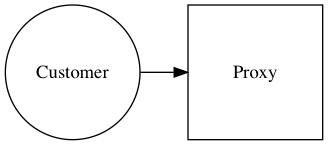
\includegraphics[width = 200pt]{sc}
%%   \caption{}
%% \end{figure}

\begin{center}
\begin{tabular}{l | l | l | l | l | l}
  ISP & Proxy & Website & P(Relate)          & P(Timing) & P(Unburn) \\
  \hline
      & x     &         & $\frac{x}{n}$      & & \\
  \hline
  x   &       & x       & $sw$               & & \\
\end{tabular}
\end{center}

It should come as no surprise that the risks in this case are quite
similar to those of VPN usage. A Chain employing no relays is
equivalent to a VPN in which a new VPN provider is selected at random
before each browsing session, and no personal information is stored by
the VPN provider.

\subsection{One Relay, One Proxy}

%% \begin{figure}[htbp]
%%   \centering
%%   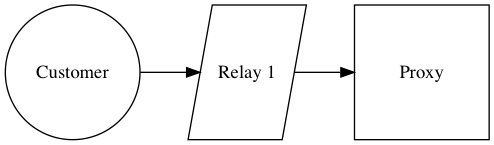
\includegraphics[width = 200pt]{stc}
%%   \caption{}
%% \end{figure}

\begin{center}
\begin{tabular}{l | l | l | l | l | l | l}
  ISP & Relay$_1$ & Proxy & Website & P(Relate)          & P(Timing) & P(Unburn) \\
  \hline
      & x         & x     &         & $(\frac{rx}{n^2})$ & & \\
  \hline
      & x         &       & x       & $w(\frac{r}{n})$   & & \\
  \hline
  x   &           & x     &         & $s(\frac{x}{n})$   & & \\
  \hline
  x   &           &       & x       &                    & $sw$ & \\
\end{tabular}
\end{center}

If bandwidth burning is employed in this configuration, all timing
attacks are mitigated. Observe that adding Relay$_1$ or the Proxy to
the Timing case allows for a Relation.

\subsection{Two Relays, One Proxy}

%% \begin{figure}[htbp]
%%   \centering
%%   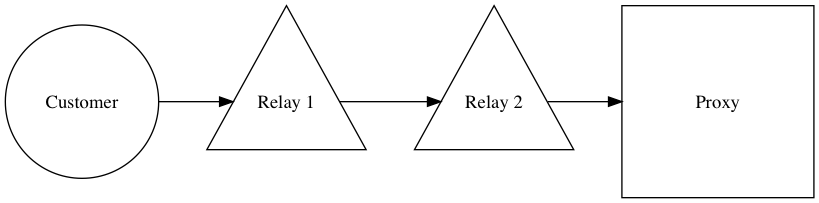
\includegraphics[width = 200pt]{sttc}
%%   \caption{}
%% \end{figure}

\begin{center}
\begin{tabular}{l | l | l | l | l | l | l | l}
  ISP & Relay$_1$ & Relay$_2$ & Proxy & Website & P(Relate)           & P(Timing) & P(Unburn) \\
  \hline
      & x         &           & x     &         & $(\frac{rx}{n^2})$  &           & \\
  \hline
  x   &           & x         & x     &         & $s(\frac{rx}{n^2})$ &           & \\
  \hline
      & x         & x         &       & x       & $w(\frac{r}{n})^2$  &           & \\
  \hline
  x   &           & x         &       & x       & $sw(\frac{r}{n})$   &           & \\
  \hline
      & x         &           &       & x       &                     & $s(\frac{r}{n})$ & \\
  \hline
  x   &           &           &       & x       &                     & $sw$      & \\
\end{tabular}
\end{center}

If bandwidth burning is employed in this configuration, all timing
attacks are mitigated. In the case of a timing attack carried out by
Relay$_1$ and the Website, adding Relay$_2$ or the Proxy to the
collusion results in a relation. In the case of the customer's ISP
colluding with the Website, adding Relay$_2$ results in a relation.

\subsection{Three Relays, One Proxy}

%% \begin{figure}[htbp]
%%   \centering
%%   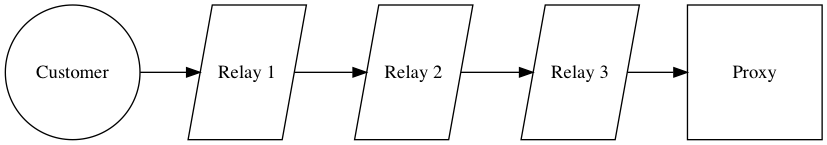
\includegraphics[width = 200pt]{stttc}
%%   \caption{}
%% \end{figure}

\begin{center}
\begin{tabular}{l | l | l | l | l | l | l | l | l}
  ISP & Relay$_1$ & Relay$_2$ & Relay$_3$ & Proxy & Website & P(Relate)             & P(Timing) & P(Unburn) \\
  \hline
      & x         & x         &           & x     &         & $(\frac{r^2x}{n^3})$  & & \\
  \hline
      & x         &           & x         & x     &         & $(\frac{r^2x}{n^3})$  & & \\
  \hline
  x   &           & x         &           & x     &         & $s(\frac{rx}{n^2})$ & & \\
  \hline
      & x         &           & x         &       & x       & $w(\frac{r}{n})^2$ & & \\
  \hline
  x   &           & x         & x         &       & x       & $sw(\frac{r}{n})^2$ & & \\
  \hline
      & x         &           &           &       & x       &                    & $s(\frac{r}{n})$ & \\
  \hline
  x   &           &           &           &       & x       &                    & $sw$ & \\
  \hline
      & x         & x         &           &       & x       &                    &      & $s(\frac{r}{n})^2$ \\
  \hline
  x   &           & x         &           &       & x       &                    &      & $sw(\frac{r}{n})$ \\
\end{tabular}
\end{center}
